\documentclass{article}
\usepackage{tikz}
\usetikzlibrary{arrows.meta,positioning,calc,shapes.geometric}
\pagestyle{empty}
\begin{document}
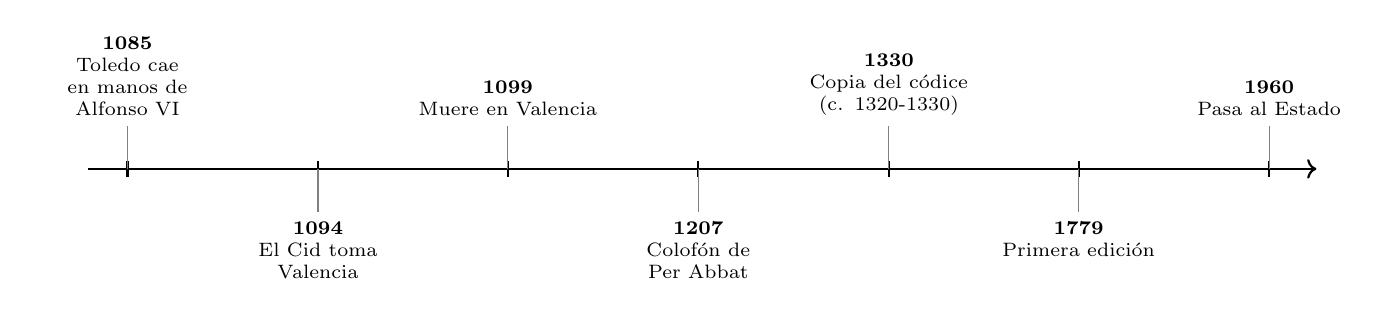
\begin{tikzpicture}
\tikzset{every node/.append style={align=center}}
\draw[->, thick] (-0.5,0) -- (15.10,0);
\draw[thick] (0.00,-0.1) -- (0.00,0.1);
\draw[gray] (0.00,0) -- (0.00,0.55);
\node[anchor=south, align=center, text width=2.30cm, font=\scriptsize] at (0.00,0.55) {\textbf{1085}\\ Toledo cae en manos de Alfonso VI};
\draw[thick] (2.42,-0.1) -- (2.42,0.1);
\draw[gray] (2.42,0) -- (2.42,-0.55);
\node[anchor=north, align=center, text width=2.30cm, font=\scriptsize] at (2.42,-0.55) {\textbf{1094}\\ El Cid toma Valencia};
\draw[thick] (4.83,-0.1) -- (4.83,0.1);
\draw[gray] (4.83,0) -- (4.83,0.55);
\node[anchor=south, align=center, text width=2.30cm, font=\scriptsize] at (4.83,0.55) {\textbf{1099}\\ Muere en Valencia};
\draw[thick] (7.25,-0.1) -- (7.25,0.1);
\draw[gray] (7.25,0) -- (7.25,-0.55);
\node[anchor=north, align=center, text width=2.30cm, font=\scriptsize] at (7.25,-0.55) {\textbf{1207}\\ Colofón de Per Abbat};
\draw[thick] (9.67,-0.1) -- (9.67,0.1);
\draw[gray] (9.67,0) -- (9.67,0.55);
\node[anchor=south, align=center, text width=2.30cm, font=\scriptsize] at (9.67,0.55) {\textbf{1330}\\ Copia del códice (c. 1320-1330)};
\draw[thick] (12.08,-0.1) -- (12.08,0.1);
\draw[gray] (12.08,0) -- (12.08,-0.55);
\node[anchor=north, align=center, text width=2.30cm, font=\scriptsize] at (12.08,-0.55) {\textbf{1779}\\ Primera edición};
\draw[thick] (14.50,-0.1) -- (14.50,0.1);
\draw[gray] (14.50,0) -- (14.50,0.55);
\node[anchor=south, align=center, text width=2.30cm, font=\scriptsize] at (14.50,0.55) {\textbf{1960}\\ Pasa al Estado};
\end{tikzpicture}
\end{document}
